\section{Purchasing and Procurement}

The Purchasing module is responsible for handling all requests for quotations (RFQs) to external vendors and converting them into formal Purchase Orders (POs) once approved.

\subsection{Viewing RFQs and POs}
Navigate to the \textbf{Purchase} app from the main dashboard. This view displays all current RFQs and POs.

\begin{figure}[H]
    \centering
    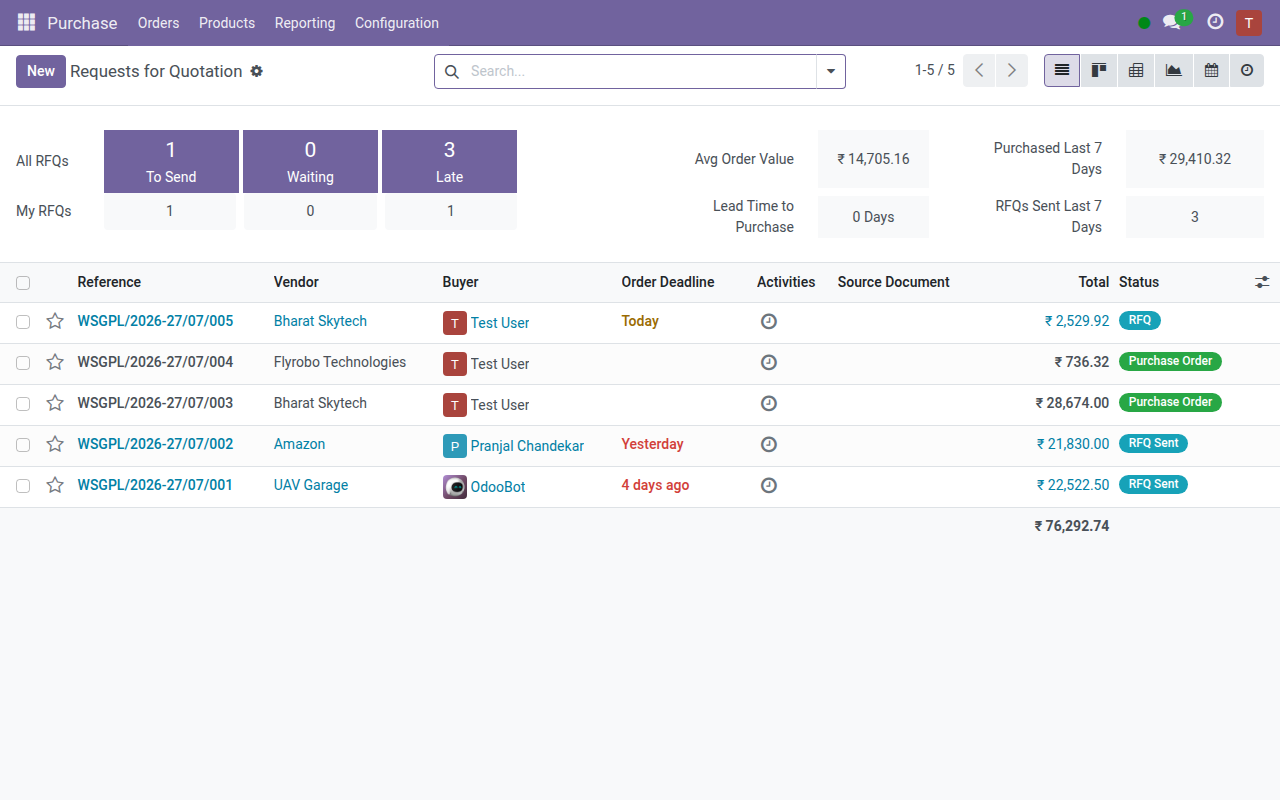
\includegraphics[width=0.9\textwidth]{images/purchase_list.png}
    \caption{Purchase Module Overview (RFQ/PO List)}
\end{figure}

\subsection{Creating a Purchase Order}
To create a new Purchase Order:
\begin{enumerate}
    \item Click the \textbf{New} button on the top-left of the Purchase overview screen.
    \item Select the \textbf{Vendor} from the dropdown list. The vendor's address and GSTIN will automatically populate in the generated PDF if they are configured correctly.
    \item Add the required products under the \textbf{Products} tab, specifying the \textbf{Quantity}, \textbf{Unit Price}, and \textbf{Taxes}.
\end{enumerate}

\begin{figure}[H]
    \centering
    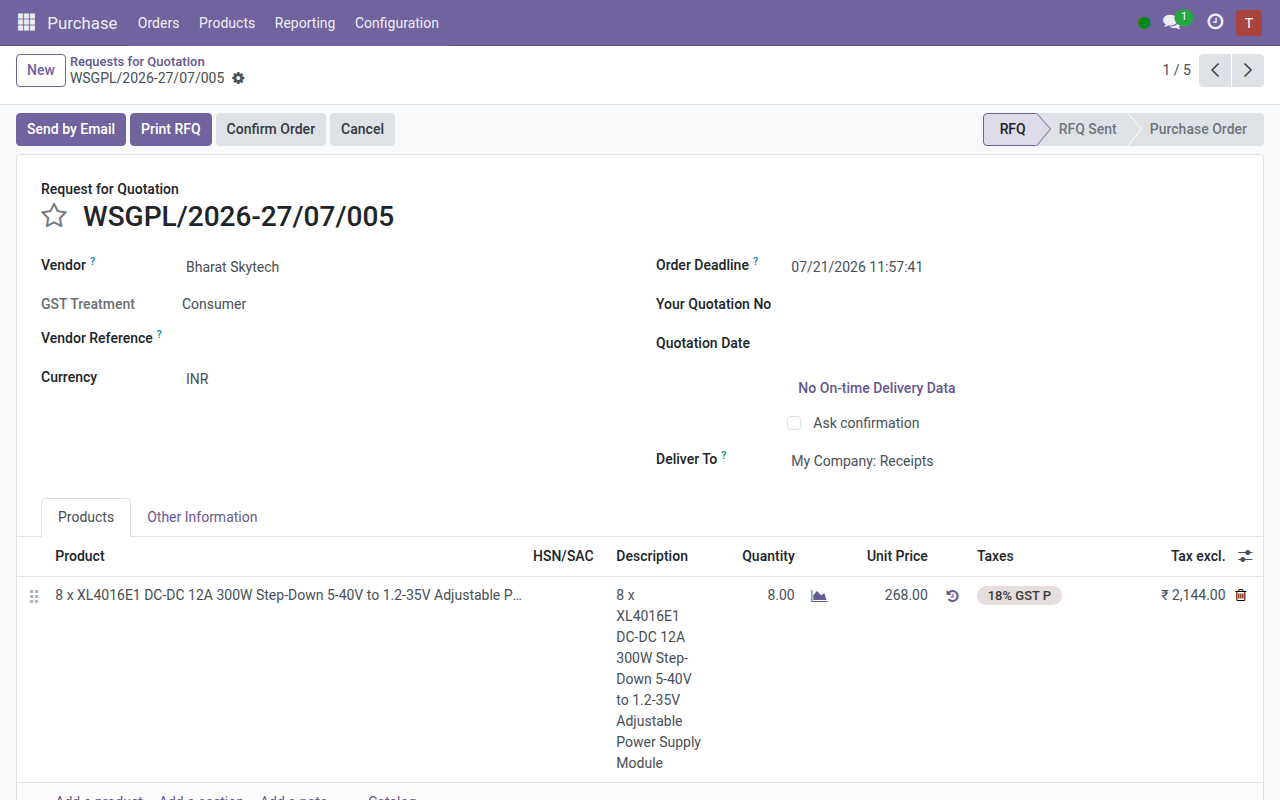
\includegraphics[width=0.9\textwidth]{images/purchase_order.png}
    \caption{Purchase Order Form View}
\end{figure}

\subsection{Printing the Official Purchase Order}
Once the RFQ has been confirmed, a custom Wingspann Purchase Order PDF can be generated.
\begin{itemize}
    \item Click the \textbf{Print} menu (gear icon) at the top of the form.
    \item Select \textbf{Purchase Order}.
\end{itemize}

\begin{notebox}
    The printed PO automatically includes the Wingspann header, standard Terms \& Conditions, and the specialized multi-tier signature block (Prepared By, Finance, Verified By, Directors) as per company policy.
\end{notebox}

\newpage
